% !TEX TS-program = XeLaTeX
% !TeX program = xelatex

\documentclass[10pt,a4paper]{article}
\usepackage[a4paper,left=15mm,right=15mm,top=18mm,bottom=18mm]{geometry}

\usepackage{minted}
\usepackage{booktabs}
\usepackage[table]{xcolor}
\usepackage{pgfplots}
\usepackage{hyperref}
\usepackage{fancyhdr}
\usepackage{abstract}
\usepackage{enumitem}
\usepackage{microtype}
\usepackage{siunitx}
\pgfplotsset{compat=1.18}

% --- siunitx setup (nice numbers + units) ---
\DeclareSIUnit{\edge}{edge}
\sisetup{
	detect-all,
	group-separator={,},
	group-minimum-digits=4,
}

\setminted{
	linenos,
	frame=single,
	breaklines,
	autogobble,
	fontsize=\footnotesize,
	bgcolor=gray!5,
}

\hypersetup{
	colorlinks=true,
	linkcolor=black,
	filecolor=blue,
	urlcolor=blue,
}

\renewcommand{\abstractnamefont}{\normalfont\Large\bfseries}
\setlength{\absleftindent}{0pt}
\setlength{\absrightindent}{0pt}

\pagestyle{fancy}
\fancyhf{}
\fancyhead[L]{\small Parallel \& Distributed Systems}
\fancyhead[R]{\small Connected Components (MPI + OpenMP)}
\fancyfoot[C]{\thepage}
\renewcommand{\headrulewidth}{0.4pt}

\begin{document}

\begin{center}
	{\LARGE\bfseries Connected Components Detection in Large-Scale Graphs (Distributed-Memory)\par}
	\vspace{0.4cm}
	{\large \textbf{Gerasimou Dimitrios} \quad AEM: 10813\\}
	\vspace{0.25cm}
	Department of Electrical and Computer Engineering\\
	Aristotle University of Thessaloniki\\
	050: Parallel and Distributed Systems\\
	\vspace{0.25cm}
	Thessaloniki, Greece\\
	December 2025
\end{center}

\vspace{0.25cm}
\thispagestyle{empty}

\begin{abstract}
We evaluate connected components (CC) detection on massive sparse graphs using a hybrid
\textbf{MPI + OpenMP} implementation targeting distributed-memory HPC systems.
Graphs are stored in a custom binary \textbf{CSC} format and distributed by contiguous column blocks
across MPI ranks, while intra-rank work is parallelized with OpenMP.

Results show that performance is strongly workload and layout dependent.
On \textbf{com-Friendster} (\num{65608366} vertices, \num{3612134270} nonzeros), splitting a \num{128}-core node into multiple MPI ranks
reduces runtime from \SI{100.5}{\second} (1$\times$128) to \SI{29.2}{\second} (16$\times$8), a \SI{3.4}{}$\times$ improvement.
Using a balanced per-node configuration (2 ranks/node, 64 threads/rank), strong scaling reaches
\textbf{4.59$\times$ speedup (relative to 1 node)} at 8 nodes (\num{1024} cores), achieving \SI{564.7}{\mega\edge\per\second}.
In contrast, on \textbf{mawi\_201512020330} (\num{226196185} vertices, \num{480047894} nonzeros), the best runtime occurs on a single node
(\SI{5.83}{\second}), while scaling to 8 nodes slows to \SI{10.54}{\second} (0.55$\times$ speedup relative to 1 node),
indicating that communication and synchronization overheads dominate for this workload in the current implementation.
\end{abstract}

\section{Introduction}
Connected components (CC) partition a graph into maximal sets of mutually reachable vertices and are a
core primitive in graph analytics (community structure, connectivity testing, preprocessing for other algorithms).
On modern machines, CC can be accelerated with shared-memory parallelism; however, real-world graphs may exceed
single-node memory capacity or be limited by memory bandwidth and NUMA effects, motivating distributed-memory designs.

This report studies a hybrid \textbf{MPI + OpenMP} CC implementation.
The emphasis is practical: (i) how graph distribution affects performance, (ii) how intra-node layout (ranks vs threads)
changes runtime even at fixed cores, and (iii) when scaling out to more nodes helps or hurts.

\section{Graph Representation and Distribution}
Graphs are represented as a binary \textbf{Compressed Sparse Column (CSC)} structure.
Only adjacency is stored; any non-zero numeric values are treated as $1$.

\begin{minted}{c}
typedef struct {
        uint32_t  nrows, ncols;  /* vertices */
        size_t    nnz;           /* edges / nonzeros */
        uint32_t *col_ptr;       /* ncols + 1 */
        uint32_t *row_idx;       /* nnz */
} CSCBinaryMatrix;
\end{minted}

For distributed execution, each MPI rank owns a contiguous range of columns (a \emph{column-block} partition).
This design is convenient for CSC because it (i) preserves sequential access patterns in \texttt{col\_ptr}/\texttt{row\_idx},
(ii) keeps per-rank adjacency compact, and (iii) provides simple ownership rules for vertex labels.

\section{Hybrid Distributed CC Method}
The implementation follows an iterative label-propagation style structure adapted to distributed memory:

\begin{enumerate}[leftmargin=*, itemsep=2pt, topsep=2pt]
	\item \textbf{Initialization:} each vertex label is initialized to its global id.
	\item \textbf{Local relaxation:} each rank scans its local CSC columns and performs label relaxations in parallel (OpenMP).
	\item \textbf{Boundary exchange:} updates affecting non-local vertices are exchanged between ranks (MPI).
	\item \textbf{Convergence check:} a global reduction determines whether any label changed in the iteration.
\end{enumerate}

In this model, scalability is largely driven by the ratio of useful local work (label relaxations over local adjacency)
to distributed overhead (boundary messages and global synchronizations). Graph structure and partitioning determine how
frequently non-local vertices are touched and how quickly labels converge.

\section{Experimental Setup}
All experiments were executed on the \textbf{Aristotelis} HPC cluster (system tag: \texttt{rome}) using AMD EPYC 7662 CPUs
(\num{64} cores/socket, \num{256}\,\si{\gibi\byte} memory per node). Benchmarks were run on 19 December 2025.
Reported times correspond to mean runtime as shown in figures.

\begin{table*}[t]
	\centering
	\rowcolors{2}{gray!10}{white}
	\begin{tabular}{lrr}
		\toprule
		\textbf{Dataset} & \textbf{Vertices} & \textbf{Nonzeros (nnz)} \\
		\midrule
		com-Friendster & \num{65608366} & \num{3612134270} \\
		mawi\_201512020330 & \num{226196185} & \num{480047894} \\
		\bottomrule
	\end{tabular}
	\caption{Datasets used in evaluation.}
	\label{tab:datasets}
\end{table*}

\section{Results}

\subsection{Single-node OpenMP scaling (1 MPI rank/node)}
Figure~\ref{fig:omp-scaling} evaluates intra-node scaling using a single MPI rank and varying OpenMP threads.
Friendster improves up to 32 threads and then degrades sharply at 64--128 threads, consistent with increasing NUMA traffic,
memory bandwidth contention, and reduced locality at high thread counts.
MAWI shows mild gains up to 64 threads and also degrades at 128 threads.


\begin{figure*}[h]
\centering
\begin{minipage}[t]{0.49\textwidth}
\centering
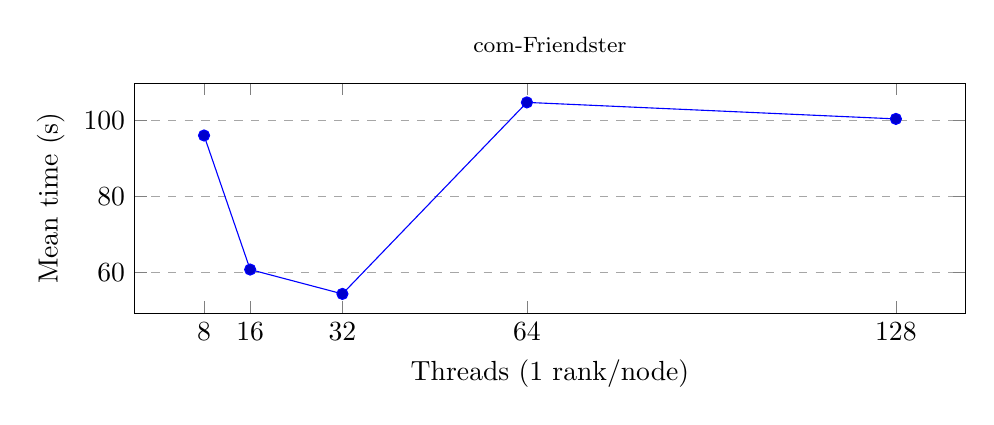
\begin{tikzpicture}
\begin{axis}[
	width=\linewidth,
	height=4.5cm,
	title={com-Friendster},
	title style={at={(0.5,1.02)}, anchor=south, font=\footnotesize},
	xlabel={Threads (1 rank/node)},
	ylabel={Mean time (s)},
	xtick={8,16,32,64,128},
	scaled x ticks=false,
	xticklabel style={/pgf/number format/fixed},
	ymajorgrids=true,
	grid style={dashed, black!35},
	mark options={solid},
]
\addplot+[mark=*] coordinates {(8,96.116) (16,60.748) (32,54.324) (64,104.843) (128,100.488)};
\end{axis}
\end{tikzpicture}
\end{minipage}
\hfill
\begin{minipage}[t]{0.49\textwidth}
\centering
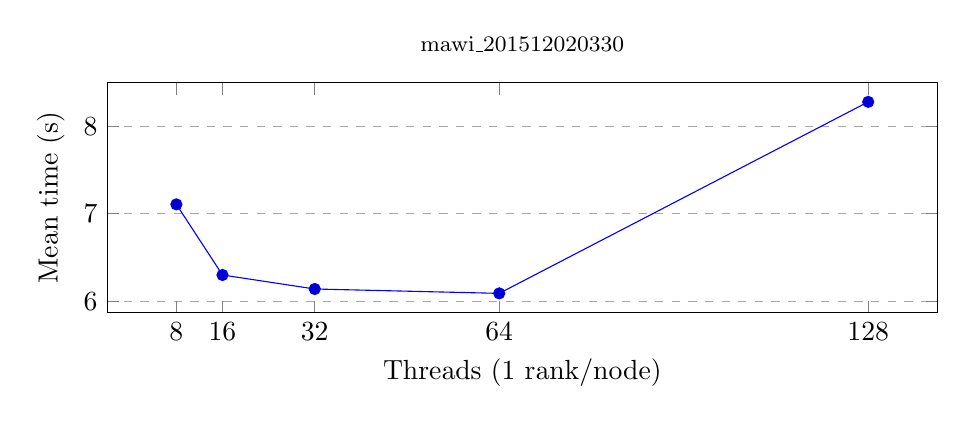
\begin{tikzpicture}
\begin{axis}[
	width=\linewidth,
	height=4.5cm,
	title={mawi\_201512020330},
	title style={at={(0.5,1.02)}, anchor=south, font=\footnotesize},
	xlabel={Threads (1 rank/node)},
	ylabel={Mean time (s)},
	xtick={8,16,32,64,128},
	scaled x ticks=false,
	xticklabel style={/pgf/number format/fixed},
	ymajorgrids=true,
	grid style={dashed, black!35},
	mark options={solid},
]
\addplot+[mark=*] coordinates {(8,7.106) (16,6.299) (32,6.139) (64,6.089) (128,8.277)};
\end{axis}
\end{tikzpicture}
\end{minipage}
\vspace{-6pt}
\caption{OpenMP-only scaling on 1 node using 1 MPI rank (time vs threads).}
\label{fig:omp-scaling}
\end{figure*}

\subsection{Intra-node layout: splitting 128 cores into MPI ranks}
Keeping a node fixed at \num{128} total cores, Figure~\ref{fig:rank-splitting} shows the effect of splitting the node into multiple MPI ranks.
Friendster benefits substantially: runtime drops from \SI{100.5}{\second} (1$\times$128) to about \SI{29}{\second} for 2--16 ranks with fewer threads/rank.
MAWI exhibits a weaker optimum near 2 ranks $\times$ 64 threads.


\begin{figure*}[h]
\centering
\begin{minipage}[t]{0.49\textwidth}
\centering
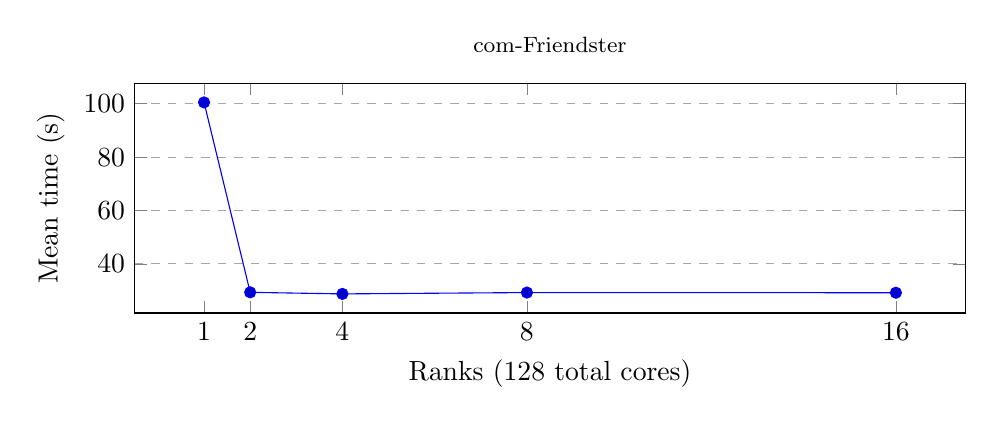
\begin{tikzpicture}
\begin{axis}[
	width=\linewidth,
	height=4.5cm,
	title={com-Friendster},
	title style={at={(0.5,1.02)}, anchor=south, font=\footnotesize},
	xlabel={Ranks (128 total cores)},
	ylabel={Mean time (s)},
	xtick={1,2,4,8,16},
	xticklabels={1,2,4,8,16},
	log ticks with fixed point,
	scaled x ticks=false,
	ymajorgrids=true,
	grid style={dashed, black!35},
	mark options={solid},
]
\addplot+[mark=*] coordinates {(1,100.488) (2,29.354) (4,28.766) (8,29.270) (16,29.204)};
\end{axis}
\end{tikzpicture}
\end{minipage}
\hfill
\begin{minipage}[t]{0.49\textwidth}
\centering
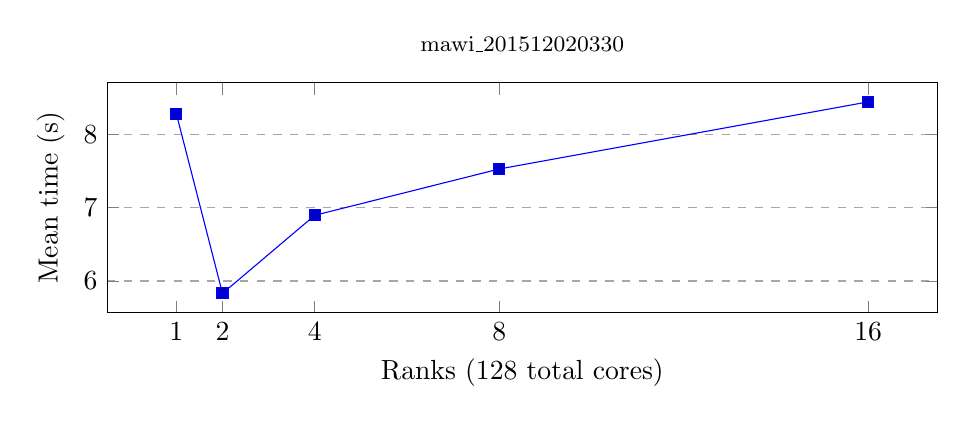
\begin{tikzpicture}
\begin{axis}[
	width=\linewidth,
	height=4.5cm,
	title={mawi\_201512020330},
	title style={at={(0.5,1.02)}, anchor=south, font=\footnotesize},
	xlabel={Ranks (128 total cores)},
	ylabel={Mean time (s)},
	xtick={1,2,4,8,16},
	xticklabels={1,2,4,8,16},
	log ticks with fixed point,
	scaled x ticks=false,
	ymajorgrids=true,
	grid style={dashed, black!35},
	mark options={solid},
]
\addplot+[mark=square*] coordinates {(1,8.277) (2,5.832) (4,6.895) (8,7.526) (16,8.440)};
\end{axis}
\end{tikzpicture}
\end{minipage}
\vspace{-6pt}
\caption{Effect of rank splitting at \num{128} total cores (1 node): mean time vs ranks/node.}
\label{fig:rank-splitting}
\end{figure*}

\subsection{Strong scaling with the recommended per-node configuration}
For strong scaling we use the best-performing per-node configuration from benchmarking:
(2 MPI ranks/node, 64 threads/rank).
Figure~\ref{fig:strong-scaling} reports speedup relative to the 1-node baseline, alongside an ideal linear reference.
Friendster scales to 8 nodes (4.59$\times$ relative to 1 node), while MAWI shows slowdowns (speedup $<1$) as nodes increase.


\begin{figure}[h]
\centering
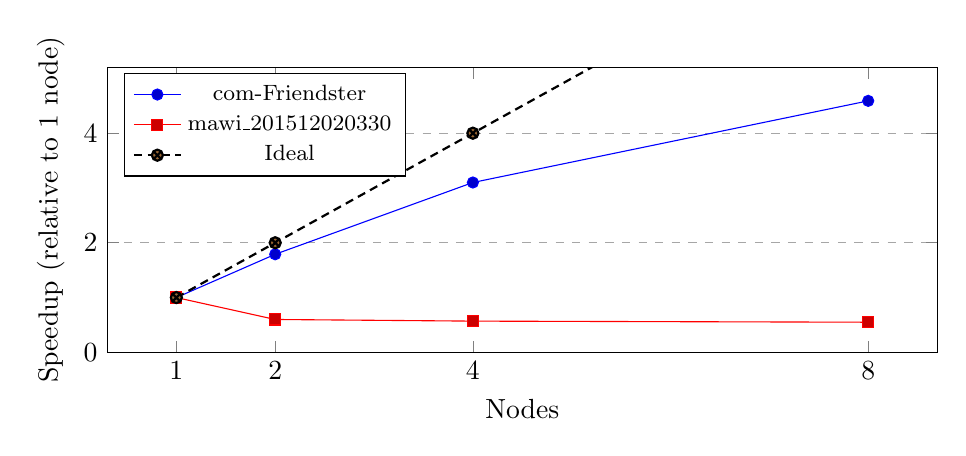
\begin{tikzpicture}
\begin{axis}[
	width=\linewidth,
	height=5.2cm,
	xlabel={Nodes},
	ylabel={Speedup (relative to 1 node)},
	xtick={1,2,4,8},
	ymin=0,
	ymax=5.2,
	ymajorgrids=true,
	grid style={dashed, black!35},
	legend style={at={(0.02,0.98)}, anchor=north west, font=\footnotesize},
	mark options={solid},
]
\addplot+[mark=*] coordinates {(1,1.00) (2,1.79) (4,3.10) (8,4.59)};
\addplot+[mark=square*] coordinates {(1,1.00) (2,0.60) (4,0.57) (8,0.55)};
\addplot+[black, densely dashed, thick] coordinates {(1,1) (2,2) (4,4) (8,8)};
\legend{com-Friendster, mawi\_201512020330, Ideal}
\end{axis}
\end{tikzpicture}
\vspace{-6pt}
\caption{Strong scaling speedup using 2 ranks/node and 64 threads/rank.}
\label{fig:strong-scaling}
\end{figure}

\begin{table*}[h]
	\centering
	\rowcolors{2}{gray!10}{white}
	\begin{tabular}{lrrr}
		\toprule
		\textbf{Dataset} & \textbf{Best 1-node time} & \textbf{8-node speedup (vs 1 node)} & \textbf{8-node throughput} \\
		\midrule
		com-Friendster & \SIrange{28.77}{29.35}{\second} & 4.59$\times$ & \SI{564.7}{\mega\edge\per\second} \\
		mawi\_201512020330 & \SI{5.83}{\second} & 0.55$\times$ & \SI{45.5}{\mega\edge\per\second} \\
		\bottomrule
	\end{tabular}
	\caption{Summary of key outcomes. Throughput is reported in million nonzeros processed per second.}
	\label{tab:summary}
\end{table*} \vspace{-0.2cm}

\section{Analysis and Discussion}

\paragraph{Friendster: layout-sensitive, then scales well.}
With 1 rank/node, Friendster degrades beyond 32 threads.
However, splitting the same \num{128} cores into multiple ranks stabilizes runtime around \SI{29}{\second}.
A likely explanation is improved NUMA locality and reduced shared-memory contention: smaller per-rank working sets and
more localized memory allocation can reduce cross-socket traffic and bandwidth pressure.
Scaling out is then effective because the per-rank workload remains large enough to amortize distributed overhead.

\paragraph{MAWI: insufficient work per rank to amortize overhead.}
MAWI has far fewer nonzeros per vertex than Friendster: roughly \num{480047894}/\num{226196185} $\approx$ \num{2.12} nnz/vertex,
compared to Friendster's \num{3612134270}/\num{65608366} $\approx$ \num{55.1} nnz/vertex.
With less local work per iteration, the fixed costs of boundary exchanges and global convergence checks become dominant.
As a result, distributing MAWI across more nodes increases synchronization and communication relative to computation,
producing a net slowdown in the current design.

Overall, the results support a practical rule: \emph{hybrid tuning is workload-dependent}.
The ranks-per-node choice can be as important as the node count, and scaling out is beneficial only when computation per rank
is large enough to hide distributed overhead.

\section{Conclusions}
We evaluated a distributed-memory connected components implementation using MPI + OpenMP on two large graphs.
Friendster benefits strongly from intra-node rank splitting and achieves \textbf{4.59$\times$} speedup at 8 nodes relative to
the 1-node baseline under a balanced layout (2 ranks/node, 64 threads/rank).
MAWI achieves its best runtime on one node and slows down when distributed, suggesting that overheads dominate for this workload
in the current implementation.

\subsection*{Future Directions}
\begin{itemize}[leftmargin=*, itemsep=2pt, topsep=2pt]
	\item Reduce communication volume (ghost vertices, compact update encoding, or selective boundary propagation).
	\item Improve partitioning quality (edge-balanced or communication-aware decompositions beyond simple column blocks).
	\item Reduce global synchronization frequency (e.g., fewer/all-reduce checks or more asynchronous progress).
	\item Add instrumentation: break down time into compute, exchange, and global synchronization to localize bottlenecks.
\end{itemize}

\noindent\textbf{Code Availability:} Source code and benchmark results are available at: \url{https://github.com/dimgerasimou/pds-hw2-mpi-connected-components}.

\end{document}

